%%%%%%%%%%%%%%%%%%%%%%%%%%%%%%%%%%%%%%%%%%%%%%%%%%%%%%%%%%%%%%%%%%%%%%%%%%%%%%%%%%
\begin{frame}[fragile]\frametitle{}
\begin{center}
{\Large Statistical Testing}
\end{center}
\end{frame}

%%%%%%%%%%%%%%%%%%%%%%%%%%%%%%%%%%%%%%%%%%%%%%%%%%%
\begin{frame}[fragile]\frametitle{Tests}
\begin{center}
\includegraphics[width=\linewidth,keepaspectratio]{ttest}
\end{center}
\end{frame}

%%%%%%%%%%%%%%%%%%%%%%%%%%%%%%%%%%%%%%%%%%%%%%%%%%%%%%%%%%%
\begin{frame}[fragile]\frametitle{Test Hypothesis}
\begin{center}
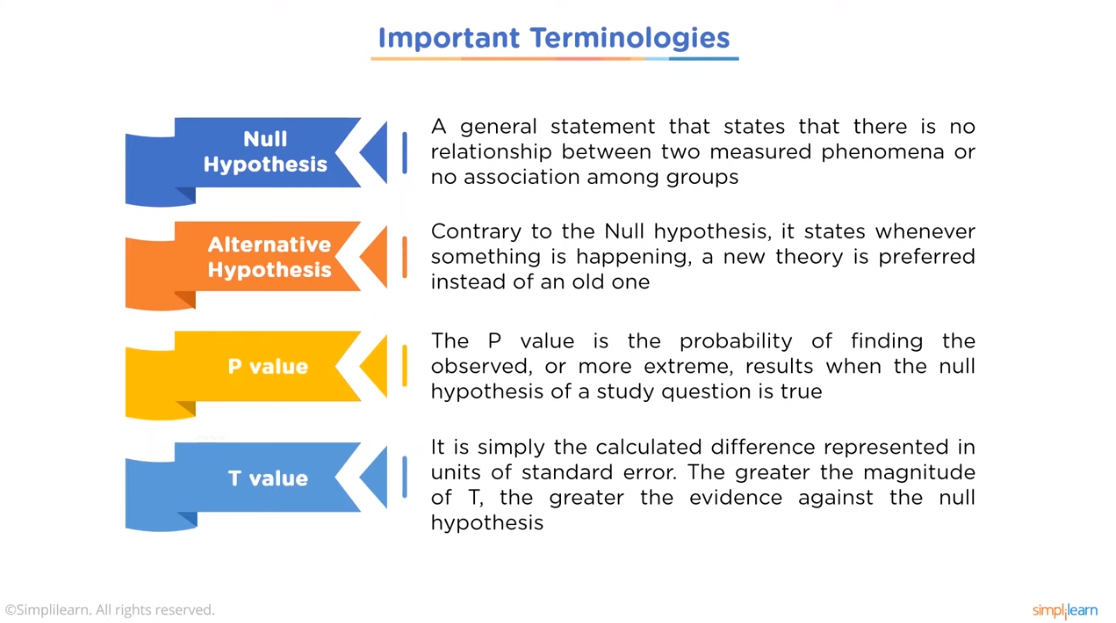
\includegraphics[width=0.9\linewidth,keepaspectratio]{stats4}
\end{center}

{\tiny (Ref: Mathematics For Machine Learning | Essential Mathematics - Machine Learning Tutorial | Simplilearn)}

\end{frame}



%%%%%%%%%%%%%%%%%%%%%%%%%%%%%%%%%%%%%%%%%%%%%%%%%%%%%%%%%%%
\begin{frame}[fragile]\frametitle{Test Hypothesis: Example}
\begin{center}
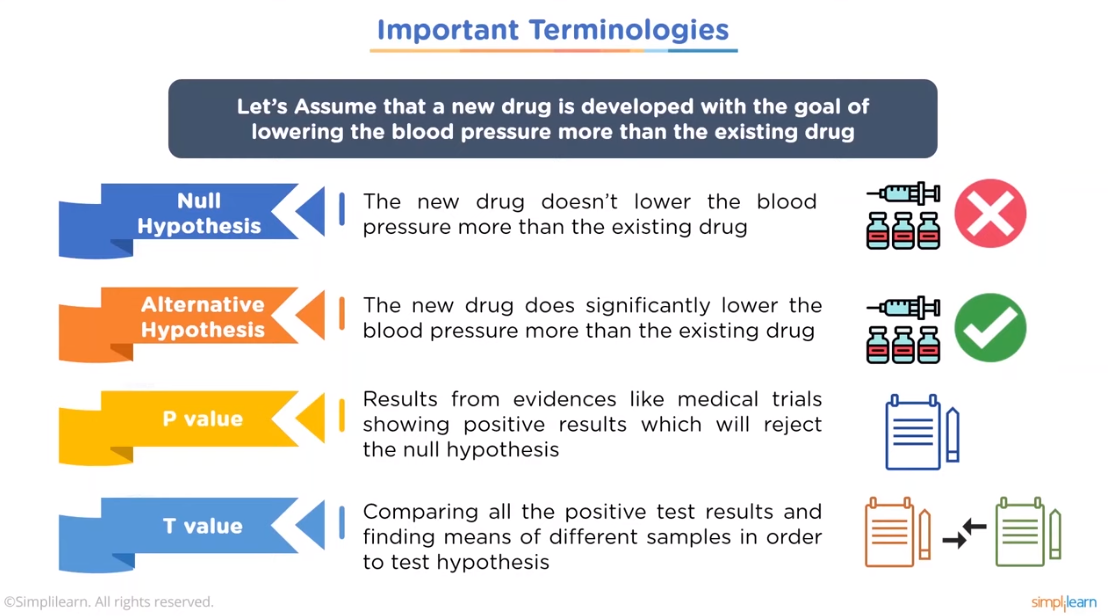
\includegraphics[width=0.9\linewidth,keepaspectratio]{stats5}
\end{center}

{\tiny (Ref: Mathematics For Machine Learning | Essential Mathematics - Machine Learning Tutorial | Simplilearn)}

\end{frame}

%%%%%%%%%%%%%%%%%%%%%%%%%%%%%%%%%%%%%%%%%%%%%%%%%%%%%%%%%%%
\begin{frame}[fragile]\frametitle{Hypothesis}
\begin{itemize}
\item Formulate effect/relation which needs to be tested
\item Null Hypothesis ($H_0$): Assume Guess/relation does not exist.
\item Alternate Hypothesis ($H_1$): Assume Guess/relation does exist. 
\item Eg. you are trying to state that your method has positive effect and there is some change.
\end{itemize}
\end{frame}

%%%%%%%%%%%%%%%%%%%%%%%%%%%%%%%%%%%%%%%%%%%%%%%%%%%%%%%%%%%
\begin{frame}[fragile]\frametitle{Hypothesis}
\begin{itemize}
\item Objective: Prove Null Hypothesis wrong.
\item Get enough evidence to disprove the Null Hypothesis.
\item {\bf Your never prove that $H_1$ is true, you can only reject $H_0$}
\end{itemize}
\end{frame}

%%%%%%%%%%%%%%%%%%%%%%%%%%%%%%%%%%%%%%%%%%%%%%%%%%%%%%%%%%%
\begin{frame}[fragile]\frametitle{Hypothesis}
Example:
\begin{itemize}
\item There is one distribution for $H_0$. 
\item There is another distribution for $H_1$
\item Your model will give some output distribution which one needs to check if its in $H_0$s acceptance region or rejection region, and how much?
\end{itemize}
\begin{center}
\includegraphics[width=0.5\linewidth,keepaspectratio]{distdiff}
\end{center}
\end{frame}

%%%%%%%%%%%%%%%%%%%%%%%%%%%%%%%%%%%%%%%%%%%%%%%%%%%%%%%%%%%
\begin{frame}[fragile]\frametitle{Confidence Intervals}
\begin{center}
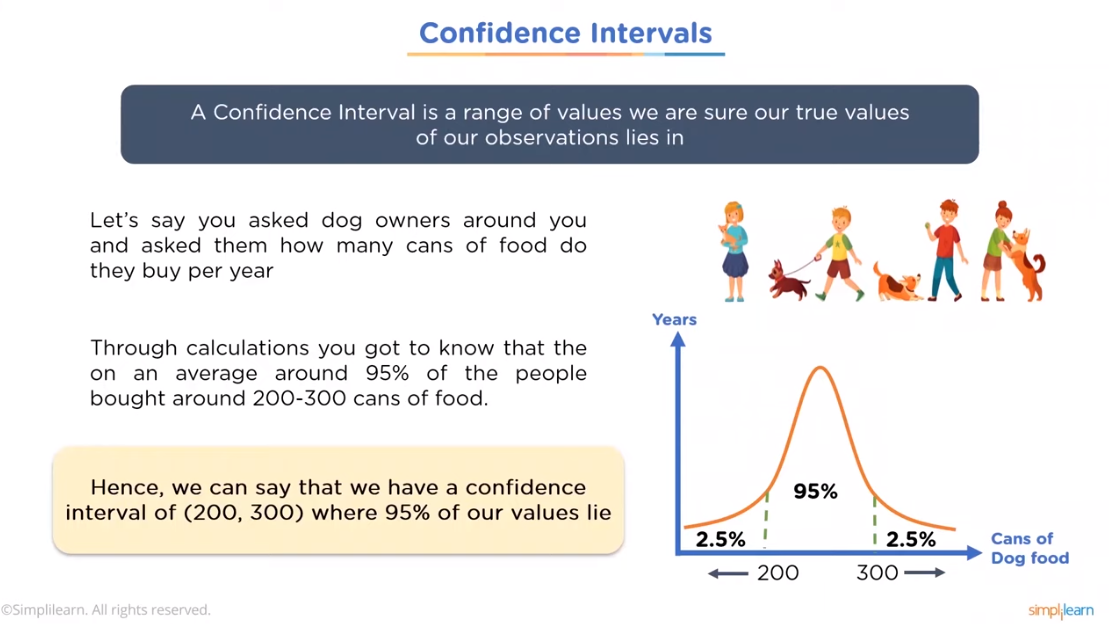
\includegraphics[width=0.9\linewidth,keepaspectratio]{stats6}
\end{center}

{\tiny (Ref: Mathematics For Machine Learning | Essential Mathematics - Machine Learning Tutorial | Simplilearn)}

\end{frame}



%%%%%%%%%%%%%%%%%%%%%%%%%%%%%%%%%%%%%%%%%%%%%%%%%%%%%%%%%%%
\begin{frame}[fragile]\frametitle{Errors}
\begin{itemize}
\item Whenever you reject a hypothesis, there is a chance that you make some errors there.
\item They care classified into Type I and Type II errors
\end{itemize}
\end{frame}

%%%%%%%%%%%%%%%%%%%%%%%%%%%%%%%%%%%%%%%%%%%%%%%%%%%%%%%%%%%
\begin{frame}[fragile]\frametitle{Errors}
\begin{itemize}
\item Type I: Incorrectly reject $H_0$. 
\item `Reject $H_0$', meaning $H_1$ can be accepted, which in turn talks about Test being positive.
\item But then `incorrectly' means Falsely , so the whole thing is False Positive.
\item Test is positive but it could actually be wrong. False Positives.
\item Probability of making Type I errors is $\alpha$
\end{itemize}
\end{frame}

%%%%%%%%%%%%%%%%%%%%%%%%%%%%%%%%%%%%%%%%%%%%%%%%%%%%%%%%%%%
\begin{frame}[fragile]\frametitle{Errors}
\begin{itemize}
\item Type II: Fail to reject $H_0$ when you should have done it. 
\item `reject $H_0$' meaning $H_1$ can be accepted, which in turn talks about Test being Positive.
\item `Fails to' do that means the Test came out negative. 
\item This should have been done, but did not happen, so `False'. So the whole thing is False Negative.
\item Test is negative but but it could actually be wrong, ie the disease is there. False Negative.
\item Probability of making Type II errors is $\beta$
\end{itemize}
\end{frame}


%%%%%%%%%%%%%%%%%%%%%%%%%%%%%%%%%%%%%%%%%%%%%%%%%%%%%%%%%%%%
%\begin{frame}[fragile]\frametitle{Some Required Definitions}
%\begin{itemize}
%\item Power: Probability of finding a difference between groups if one truly exists = $1 - \beta$. 
%\item Good to have High Power. 
%\item Having beta less that 20\%.
%\item Power increases as sample size increases, as you have more data to make conclusions.
%\item Power increases as difference between groups becomes more significant. Easy to differentiate.
%\item Power increases as precision increases (ie decrease in std deviation)
%\end{itemize}
%\end{frame}


%%%%%%%%%%%%%%%%%%%%%%%%%%%%%%%%%%%%%%%%%%%%%%%%%%%%%%%%%%%
\begin{frame}[fragile]\frametitle{Some Required Definitions}
\begin{itemize}
\item Normality: Most of the test assume that, the data or test statistics 
or some function in testing procedure under consideration follows 
Normal distribution. 
 
\item Decision  criteria: z critical values:  boundaries for rejection or non rejection region
\end{itemize}
\end{frame}
